\section{Packet-based Cortex Serial Communication}

Based on the work of the legendary work of EvolvedAwesome \cite{VEXSerial}, I propose a new method of UART communication \cite{UARTBasic} between the Raspberry Pi and the VEX Cortex.

\begin{figure}[h]
    \centering
    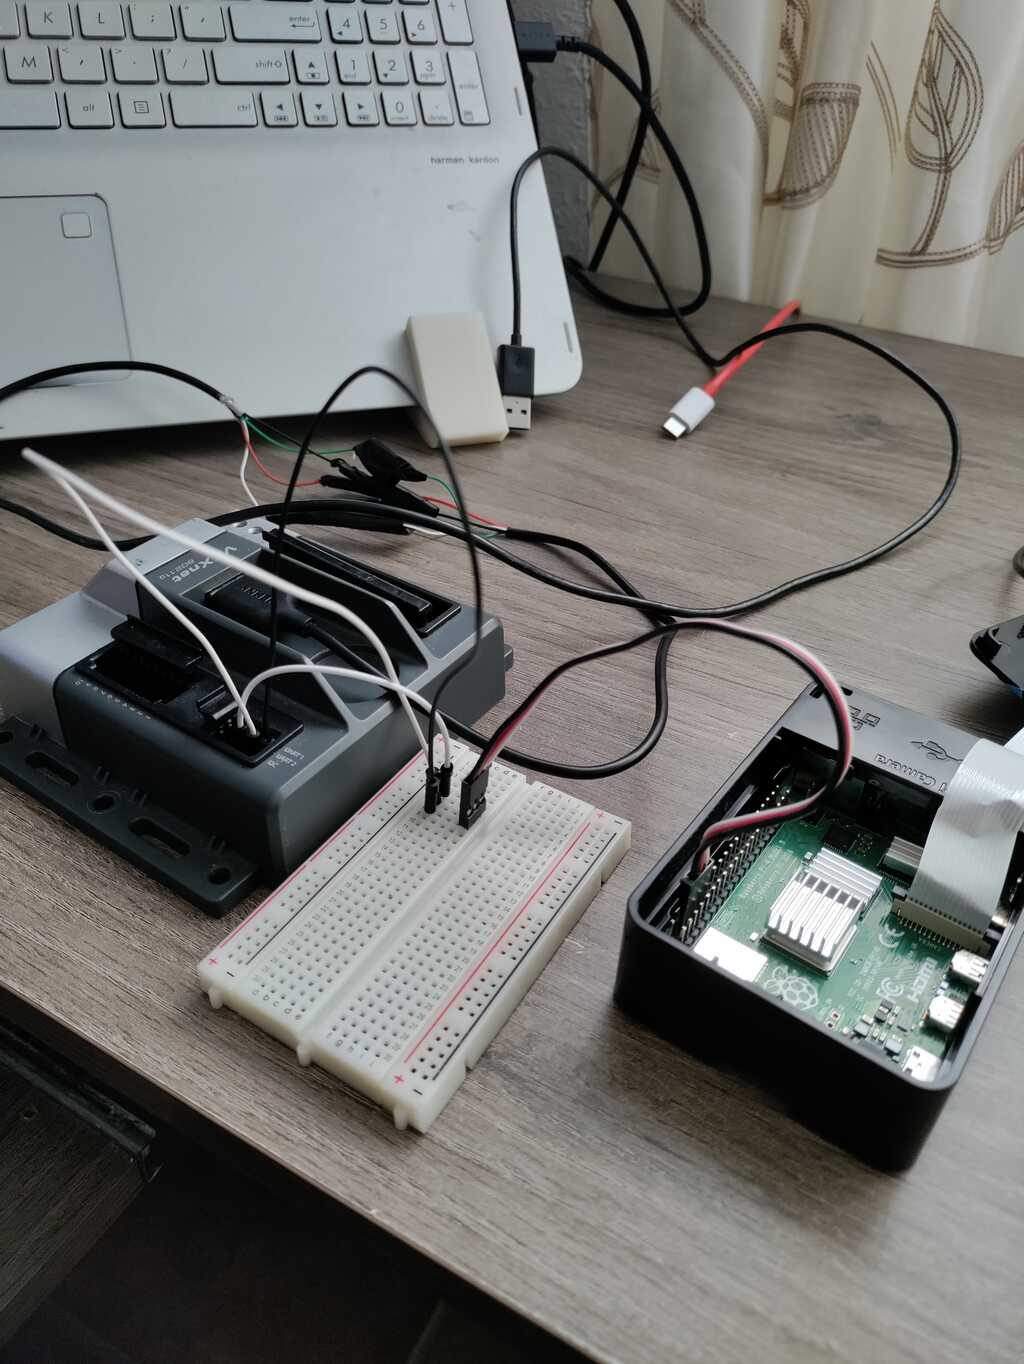
\includegraphics[width=\textwidth,height=6cm,keepaspectratio=true]{Serial/SerialSetup}
    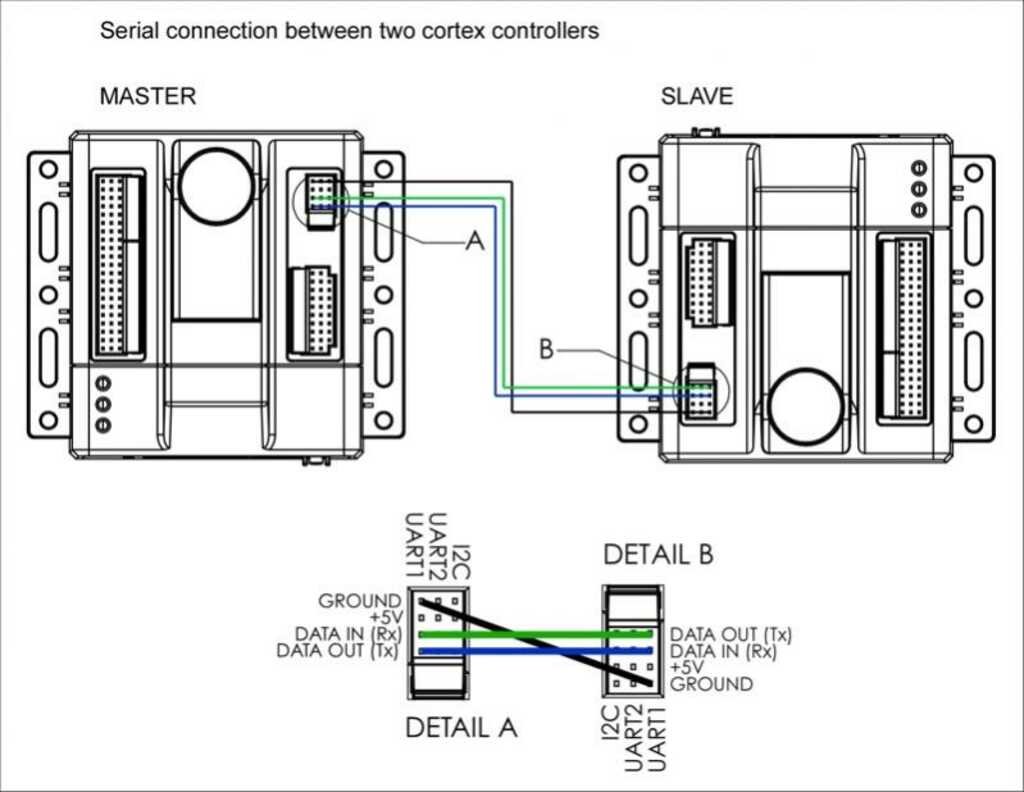
\includegraphics[width=\textwidth,height=6cm,keepaspectratio=true]{Serial/CortexWiring}
    \caption{
        (Left) The Raspberry Pi being electronically connected to the VEX Cortex via jumper wires and a breadboard. (Right) Diagram showing the UART ports of the Cortex. \cite{CortexWiringCite}
    }
\end{figure}

The VEX Cortex contains two UART serial ports for external sensors that are now defunct. Fortunately, these ports work with standard ASCII encoded bytes, so I wrote a script in python and a program in RobotC to turn a wheel every second. After hours of debugging and coding, I eventually was able establish complete two-way communication between the Cortex and the Raspberry Pi, thus unlocking limitless possibilities.

At a technical level, sending a single byte of data is useless. The maximum amount of information you'd be able to convey is a single byte that can only hold an integer between 0 - 255. Due to how UART communication works, you can't just send multiple bytes in a specific order either, as neither computer knows when each "packet" of data starts and when it ends. To solve this problem, I used EvolvedAwesome's approach of tagging the start of each packet of data with a reserved integer so the robot would be able to wait until a packet starts and when it ends. This approach is super flexible, allowing any size packet of information to be sent to the Cortex with no penalty. If a byte gets corrupted during transit, you can just program a checksum to throw the data away.

\begin{figure}[h]
    \centering

    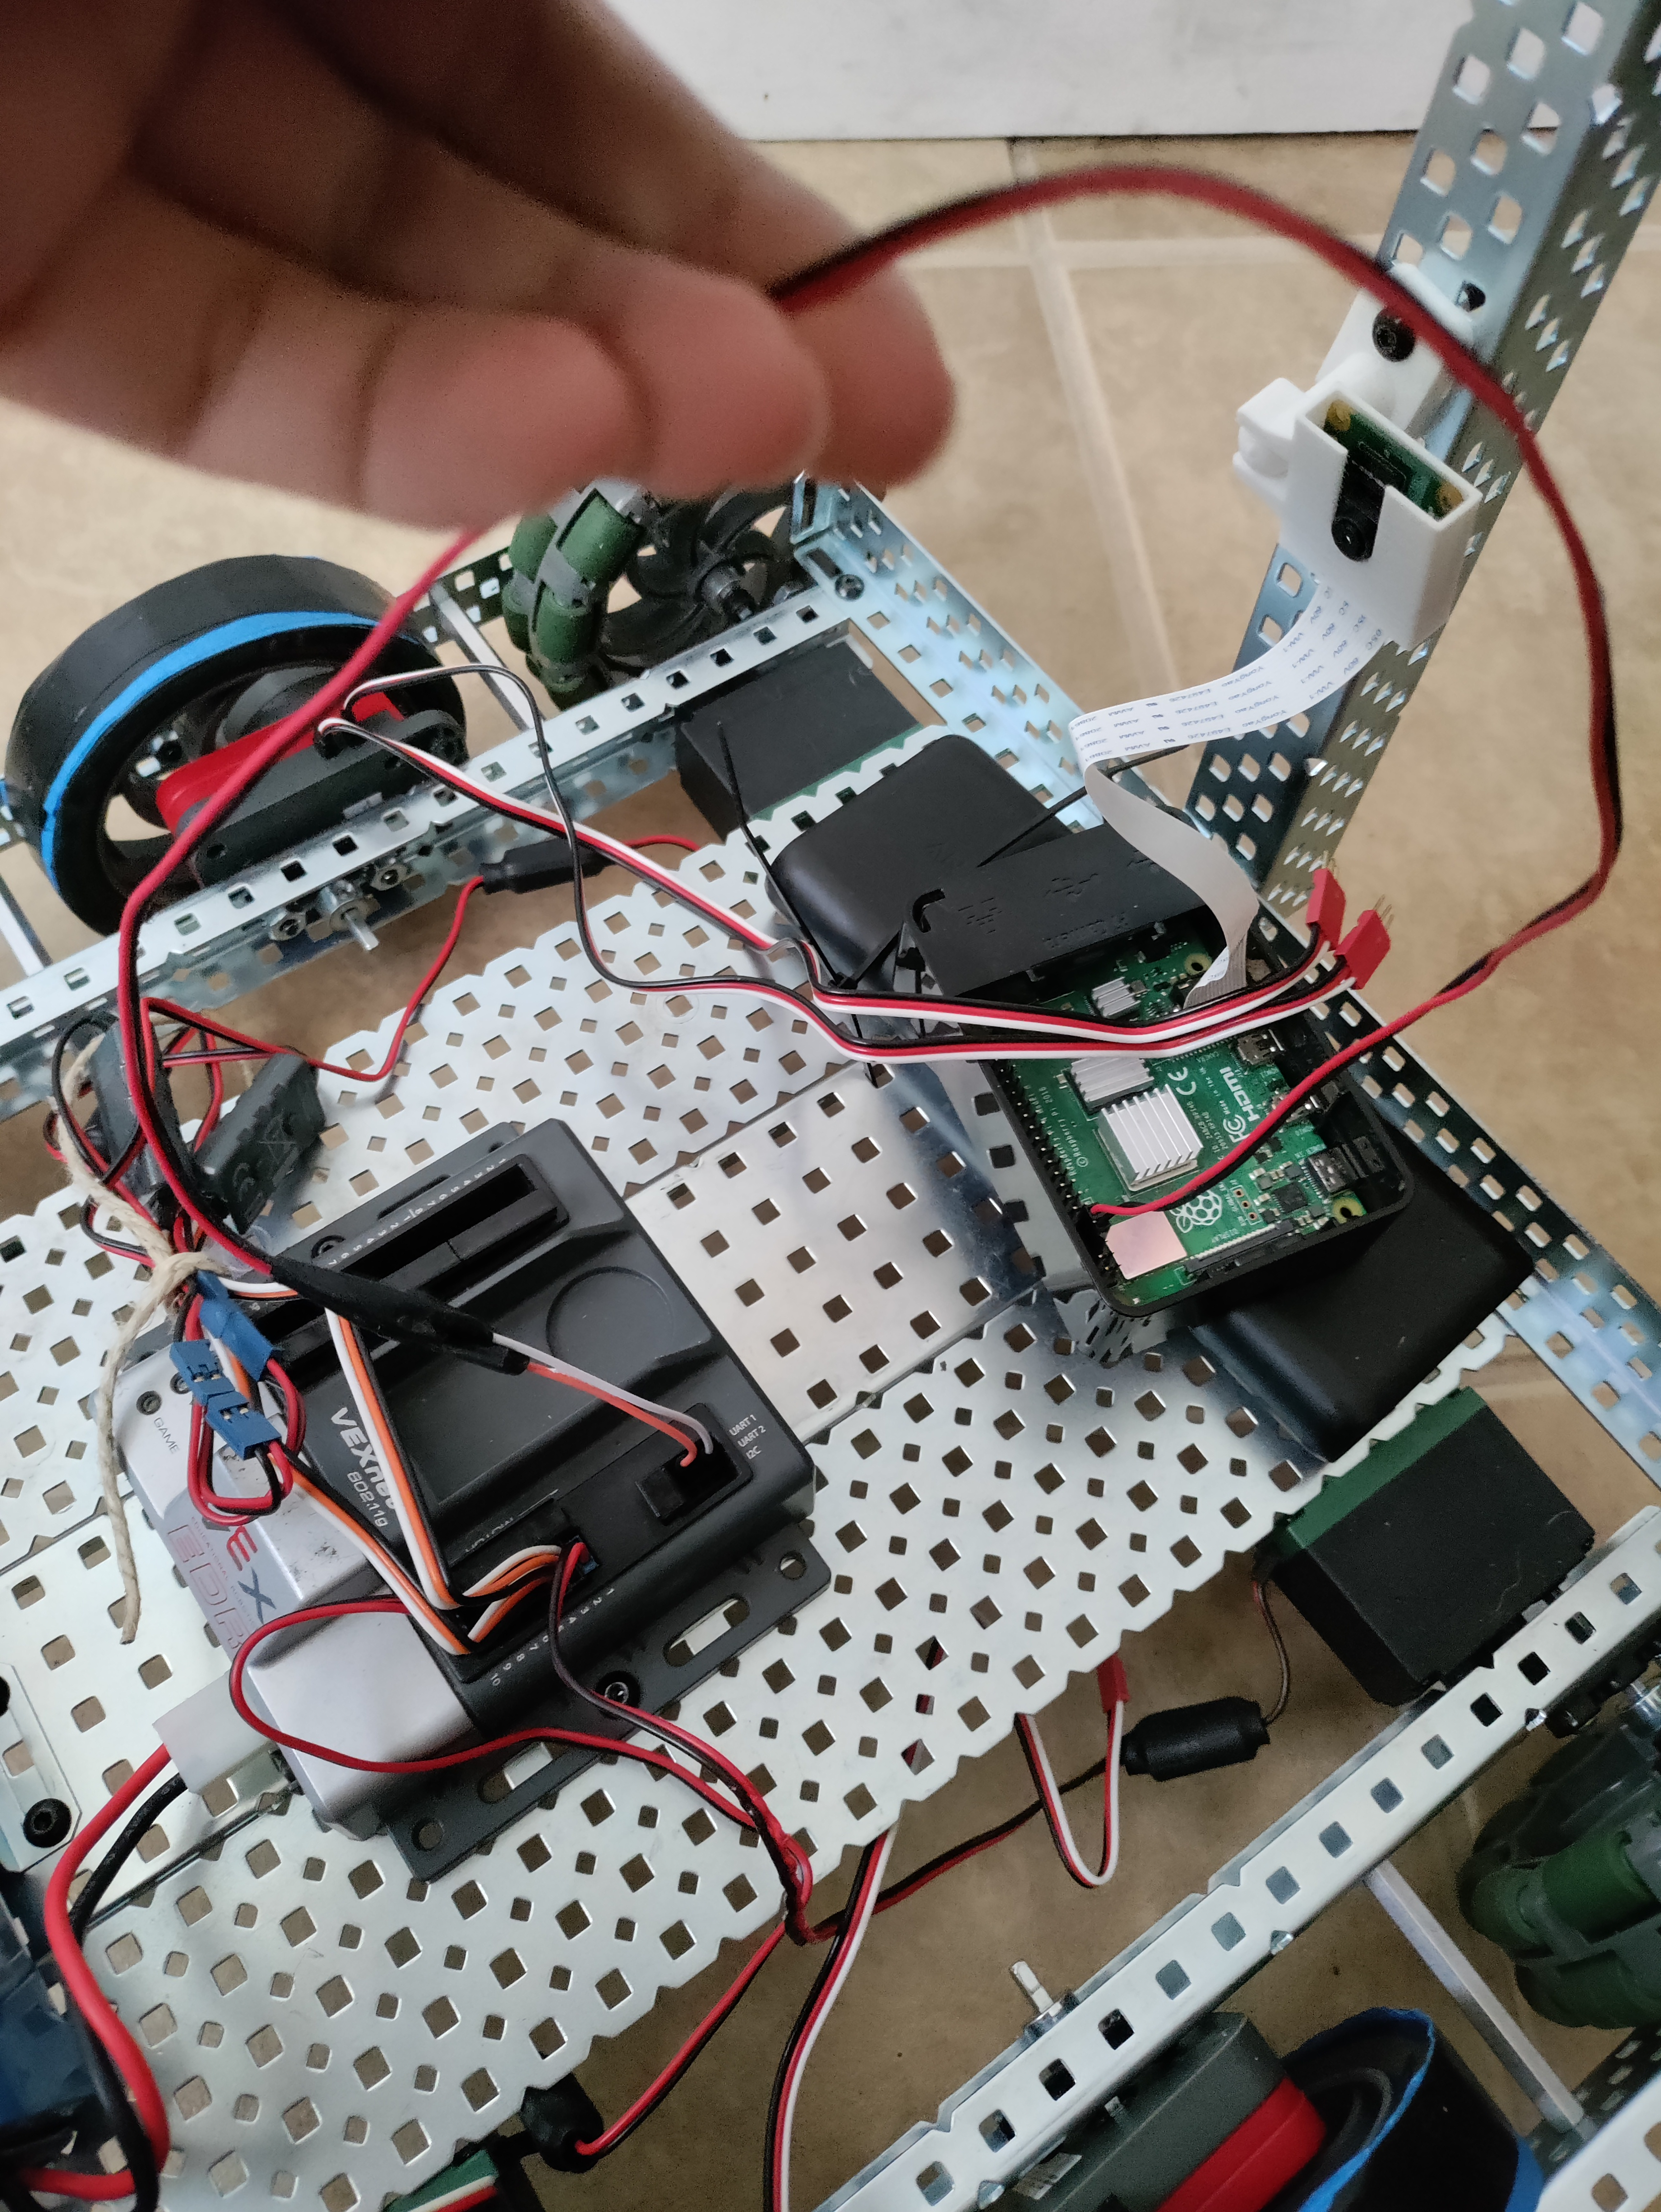
\includegraphics[width=\textwidth,height=6cm,keepaspectratio=true]{Serial/SerialMounted}
    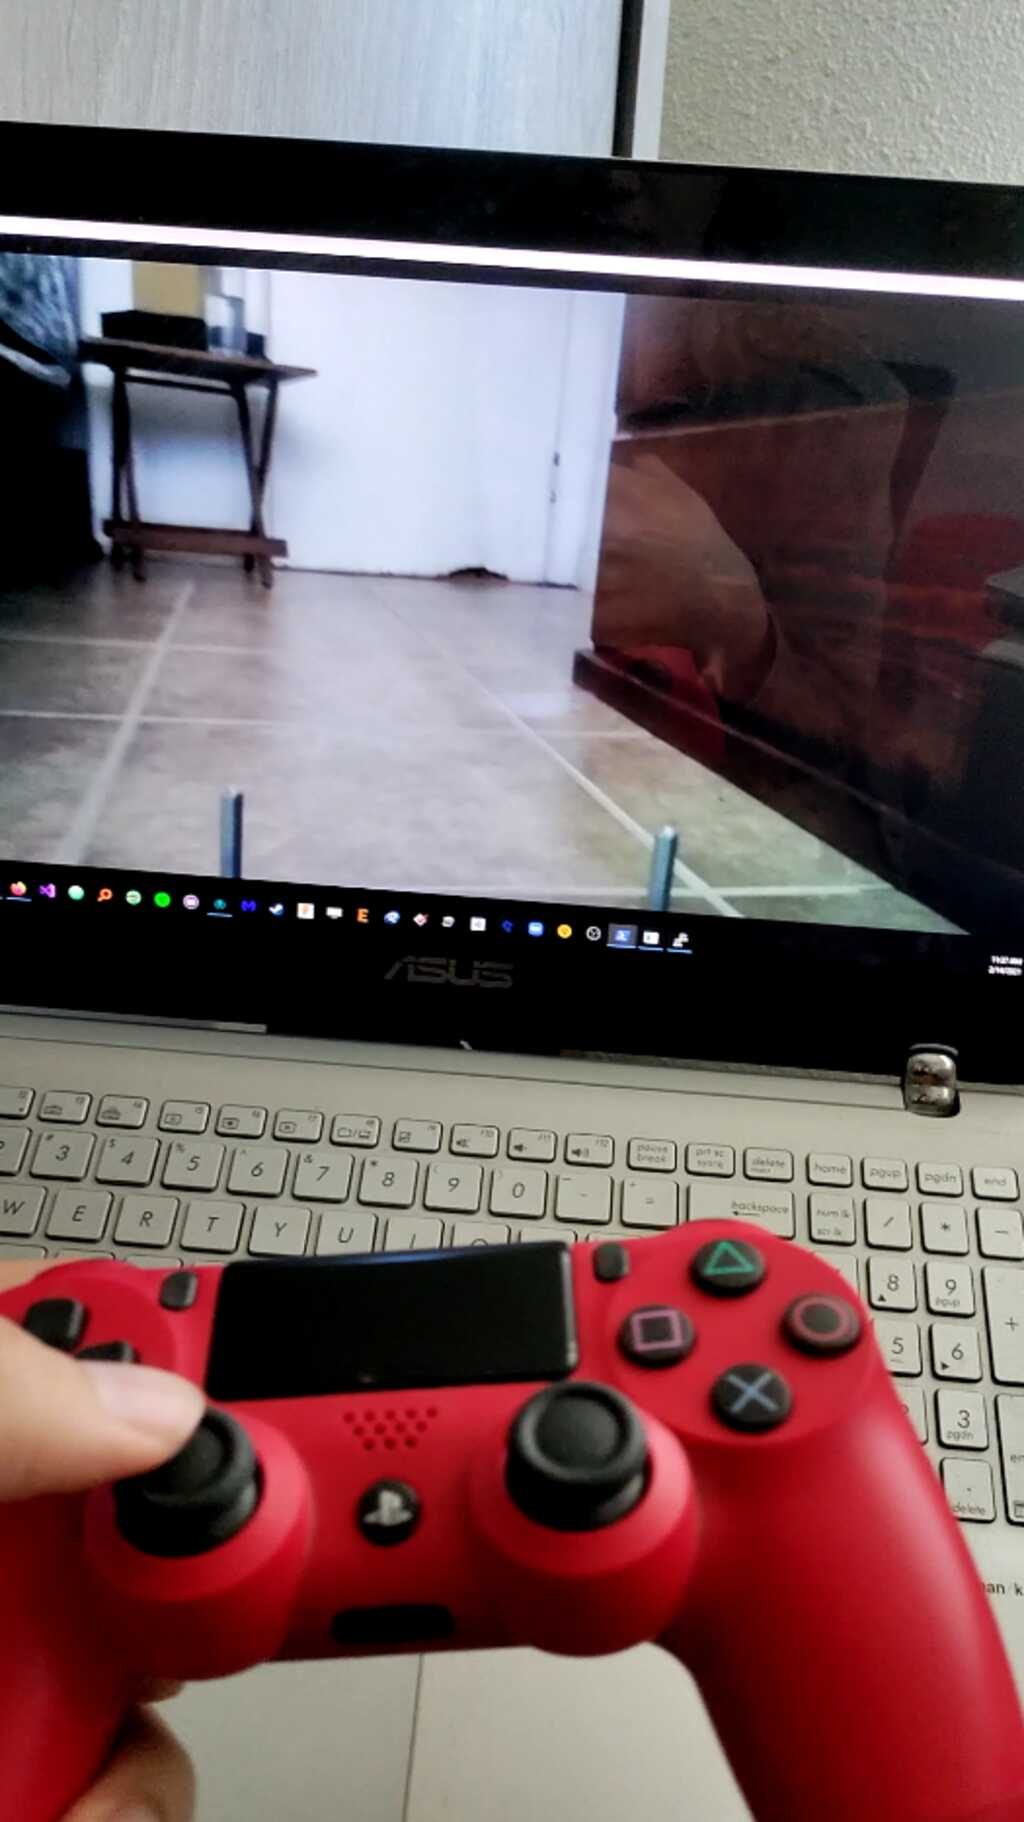
\includegraphics[width=\textwidth,height=6cm,keepaspectratio=true]{Serial/RemoteController}
    \caption {
        (Left) Cortex hooked up to the Raspberry Pi without a breadboard; The electronic link between the Raspberry Pi and Cortex was made using a homemade female to male connector. (Right) A photo of the robot being controlled by a PS4 controller with a real-time video feed.
    }
\end{figure}

One of the first things that came to mind to abuse this power was using a PS4 controller to control the VEX Cortex. In just two hours, I made a script that allowed me to control the Cortex from the comfort of my computer through UDP sockets linking the Raspberry Pi and PC together. The latency of this setup was around 33-50 ms; Not pro-gamer levels of fast, but definitely fast enough for the average user.

A lot more things can be done with this technology than just this. A high-end computer could analyze the environment real time in combination with the Wireless Camera and steer the robot. An infinite number of people can control every aspect of the robot if needed. A super-secret file on the computer can be streamed into the Cortex and act as a secret storage device. We can stream the robot on Twitch and have people pay us to steer the robot in whatever direction they please to go through an obstacle course. Control the robot from a remote location. Use the information from an industrial level gyroscope on the Raspberry Pi to achieve super accurate control on the robot. Truly, the possibilities are limitless. 


